\chapter{Continuous Integration and Continuous Delivery} \label{ch:cicd}

This notebook is mainly about Linux. In this appendix chapter, the scope of the notebook is slightly extended to software development, which is very often what Linux is used for in practice. \myabb{Continuous Integration and Continuous Delivery}{CI/CD} has become a widely adopted software development framework and philosophy, and it is introduced in this chapter.

Some contents of this chapter come from \cite{honai2023cicd}.

\section{Agile VS Waterfall}

Agile and waterfall are both project management methodologies. Both of them are introduced here, starting with the more conventional waterfall model and then followed by agile model.

\subsection{Waterfall}

Speaking of project proposal, development, testing and delivery cycle, it is fairly intuitive to follow the procedures below.
\begin{enumerate}
	\item Understand requirements from the user.
	\item Design the architecture of the solution.
	\item Develop the solution.
	\item Test the solution.
	\item Deliver the solution and close the project.
	\item (Follow-up) maintain the solution.
\end{enumerate}
The philosophy behind waterfall, as its name indicates, is to ``follow the procedures and do not turn back''. When a previous step is considered completed, it is completed and should not be revoked or revised. This is demonstrated by Fig. \ref{ch:cicd:fig:waterfall}.
\begin{figure}[htbp]
	\centering
	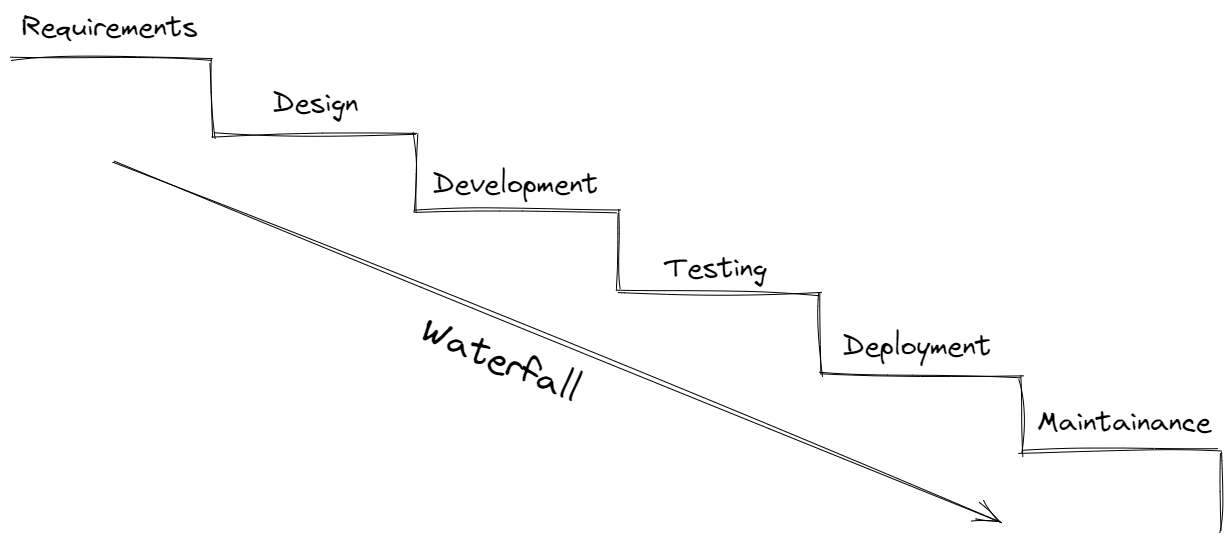
\includegraphics[width=300pt]{chapters/ap/figures/waterfall.png}
	\caption{Waterfall model.} \label{ch:cicd:fig:waterfall}
\end{figure}

With waterfall, a project can be designed, developed and deployed in a relatively efficient manner. However, there is one limitation: everything done in earlier steps cannot be changed in later steps. This sets up a high bar on both the user and the developer. For example, in step 1 ``understand requirements from the user'', the user needs to illustrate all the requirements to the developer as they cannot be modified in later steps. Similarly, in step 2 ``design the architecture'', the developer needs to optimize the design to his best, as the architecture cannot be changed later.

Regrettably, with the rapid change in the market and the aggressive advent in technology today, it is challenging even for the smartest users and developers to determine all the requirements and designs in the beginning stage of the project. More likely, the requirements of the user have to change to adapt to the market trend, and so does the technologies used in the solution.

Assume that some changes have to be made to the system. If the project development is still in an early stage, it is possible to start over. The resources already been spent are wasted. If the project development is in a late stage, it might be preferable to deploy the system with its current capability, and later add the changes to the system as new features upgrades. However, the integration often introduces a blackout period of the system. If the system is already in use, the customer experience would be affected by the blackout.

\subsection{Agile}

Agile is the counterpart of waterfall. It is proposed to tackle the aforementioned issues: rapid change of requirements and technologies during the development. It allows continuous integration and delivery of new features into the system in a convenient and consistent manner without introducing blackout.

In agile architecture, the development is modularized by features. Each feature, before deploying and integrating into the production environment, circulates in its own ``development and testing circle'', where it can be tested and reviewed iteratively by the developers and the users audit team, as shown in Fig. \ref{ch:cicd:fig:agile}.
\begin{figure}[!htb]
	\centering
	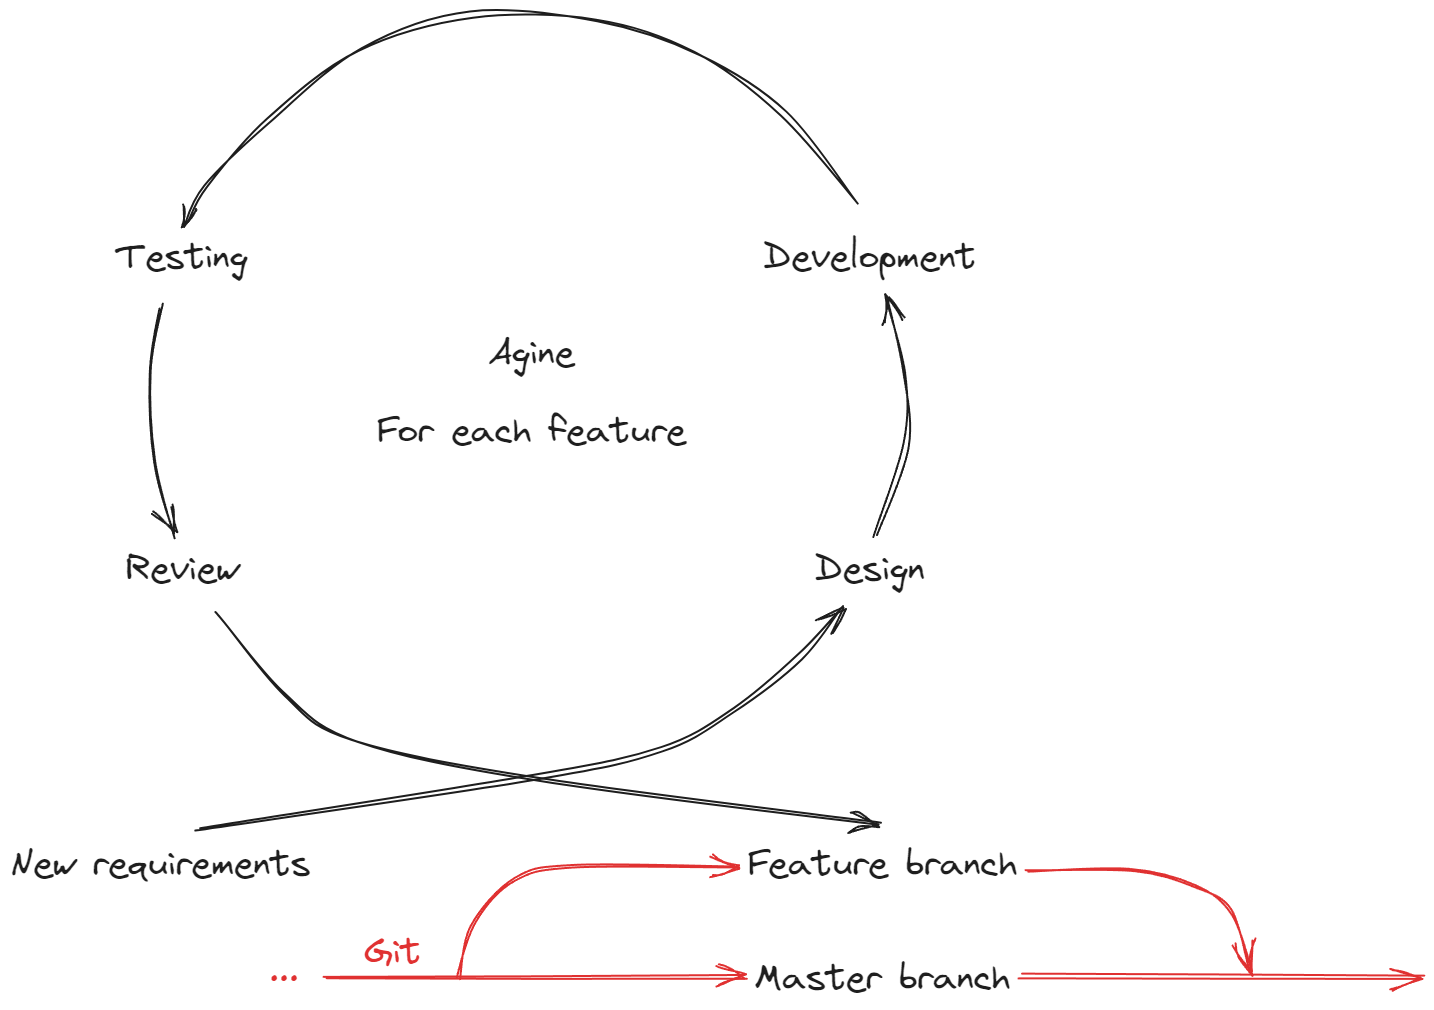
\includegraphics[width=300pt]{chapters/ap/figures/agile.png}
	\caption{Agile model.} \label{ch:cicd:fig:agile}
\end{figure}

Agile allows rapid changes to be made to the requirements and realizations of a feature. Should there be a change, just keep cycling in Fig. \ref{ch:cicd:fig:agile} until everyone is happy, before it is pushed back to the master branch.

In parallel development where there are multiple features running in their associated circles, the developer can easily choose which feature branch and circles to prioritize. This gives the developer a clearer overview of what is happening and how to best response to the customers immediate requirements.

As will be introduced later, agile is widely used in CI/CD.

\subsection{Roles in Agile-based Development}

Many roles are defined in the agile framework, each role coming with a responsibility. The roles may slightly differ for different projects. The most commonly seen set of roles known as \mync{scrum} is introduced in Table. \ref{ch:cicd:tab:agilerole}.
\begin{table}[!htb]
	\centering
	\caption{Roles in Agile model.} \label{ch:cicd:tab:agilerole}
	\begin{tabularx}{\textwidth}{lX}
		\hline
		Role & Description \\
		\hline
		Product owner & Manage the entire program. He understands all the user requirements and tracks the progresses of all the features under development. He signs off features before they are deployed. \\ \hdashline
		Scrum master & Lead the developer team as team manager or chief developer. He knows the challenges and manpower required by each feature. He sets priorities and assigns tasks to the developers. \\ \hdashline
		Developer & Based on requirements, program the features. \\ \hdashline
		Tester & Design test cases to verify the efficacy of the developed feature. \\ \hdashline
		Operator/Supporter & Maintain the software after it is delivered. \\
		\hline
	\end{tabularx}
\end{table}

In this role assignment, the product owner and scrum master come up with the product backlogs, which clarify the sprints (tasks) and their priorities. The team then knows which sprints they shall work on first.

In the case where the features concern a professional domain (such as economics, medical, etc.) that the developers do not understand, business analysts are involved. A business analyst knows both the user use cases and requirements as well as the developers' skill sets and technologies, and he bridges the user with the developers.

For each sprint, sprint planning and sprint backlog are proposed that describes the schedule of the sprint. The team works on the sprint and host daily scrum meetings until the sprint is solved. Upon finishing of a sprint, sprint review is hosted for audition.

\section{CI/CD Workflow}

\mync{Continuous Integration and Continuous Delivery}[CI/CD] is both a philosophical concept and a bunch of technologies that speeds up the development, testing and deployment cycle of a software. It has become a common and beneficial practice for collaborative projects with rapid updates.

\subsection{Pipeline}

A \mync{CI/CD pipeline} refers to the procedure a task must go through before it is delivered to the production environment. It often involves the following steps:
\begin{enumerate}
  \item Integration
  \begin{enumerate}
    \item Commit and build the branch with the new features.
    \item Test the branch.
    \item Merge the branch with the master branch.
  \end{enumerate}
  \item Delivery
  \begin{enumerate}
    \item Release the master branch to the main repository.
    \item Deploy the solution to the production environment.
  \end{enumerate}
\end{enumerate}

\subsection{Continuous Integration}

In the development of a sprint, new codes are rapidly developed, and they are rapidly built, merged and tested.

Conventionally, the integration of a new feature requires involvement from multiple parties. An example is given in Fig. \ref{ch:cicd:fig:conventionalintegration}. It includes the developer who program the software following users (or business analysts) requests, the integration team who integrates the new feature with the existing system and compile the code into packages, and the operations team who upload the new system into the pre-prod environment for real data testing, and the testers who audit the output of the program running in the pre-prod environment.

\begin{figure}[!htb]
	\centering
	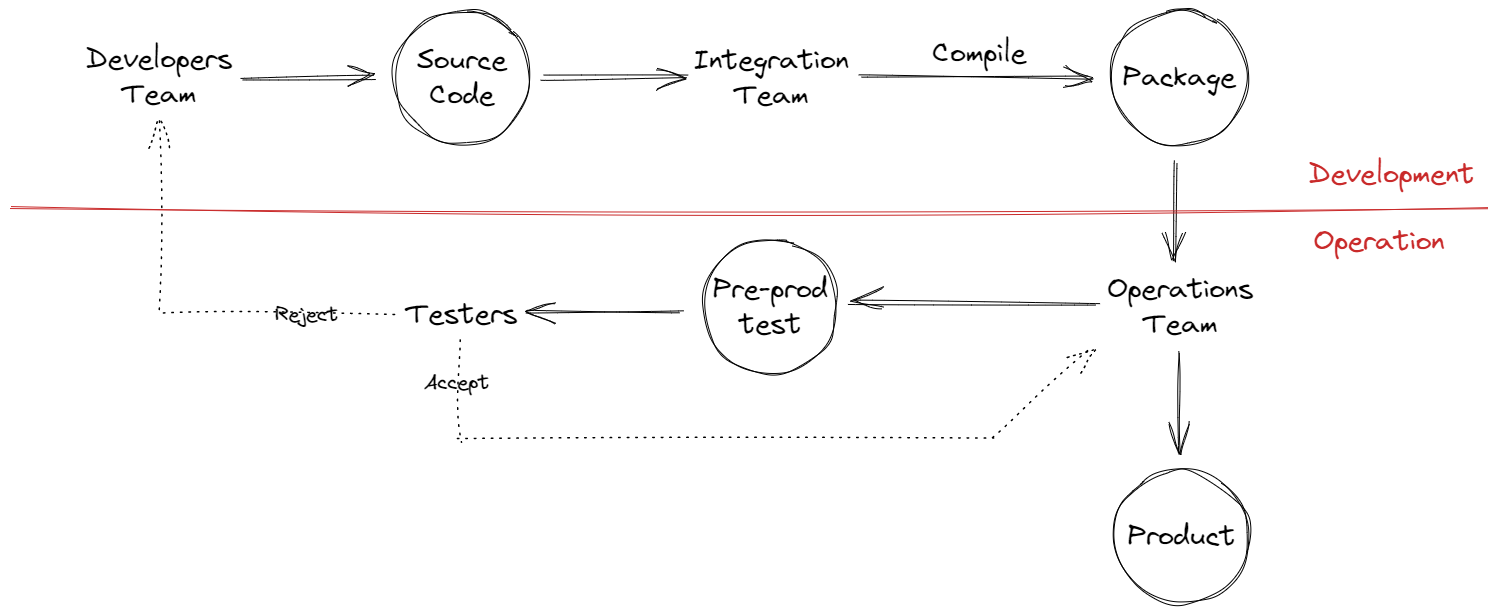
\includegraphics[width=350pt]{chapters/ap/figures/conventionalintegration.png}
	\caption{Integration and delivery of a new feature. The integration corresponds with the development and delivery, operation, in the figure respectively.} \label{ch:cicd:fig:conventionalintegration}
\end{figure}

Should there be any error along the way, the code is roll back the developer team for trouble shooting. When the new system with the updated code survives pre-prod environment, it is then pushed to the production environment.


In practice, each cycle in Fig. \ref{ch:cicd:fig:conventionalintegration} can take a few days or even weeks as so many teams have to cooperate to make it happen. It takes time for the integration team to integrate different branches in the source code together, making sure that components from different branches function properly. When there is a defect, the flaws can be spotted only in the last stage of the iteration, i.e., testing. This practically disallows very frequent update of the system in response to the rapid changes in requirements.

\myabb{Continuous Integration}{CI} (together with \myabb{Continuous Delivery}{CD} which is introduced in the later section) tries to solve the above problems. CI automates the ``development'' portion in Fig. \ref{ch:cicd:fig:conventionalintegration}, while CD automates the ``operation'' portion.

To speed up the development of new features, CI mainly adopts the following methods.
\begin{itemize}
	\item Use Git to manage features. This simplifies the procedure of managing multiple under-development features and integrating them together. Integration is now managed by Git following developers' intention.
	\item Use a build server to automatically compile the code into ready-for-delivery packages. The scrum master and senior developers can access the server and monitor the progression. Should there be a compiling error, the developer is notified immediately.
	\item The code, after compiling, is immediately tested in the build server using pre-defined test cases. If the code fails the test cases, the developer is immediately notified.
\end{itemize}

CI effectively removed ``integration team'' from the picture. The integration related tasks are split into small pieces and processed by automation tools, feature integration by Git, and compiling by build server. During CI, the developer not only generates the codes, but also supervises Git and build server. Should there be any error, the developer is notified immediately by the automation tools.

CI speeds up the developing cycle, from the receiver receiving requests from the user, to the point they have new system in the package ready for pre-prod testing.

\subsection{Continuous Delivery}

The package received from the development side contains the latest version of the system where a new feature is integrated. It is, however, not certain at this point whether the new feature works properly and how the system would behave as a whole with this new feature. The sophisticated testing and deployment of the software features are done by the operations team.

Conventionally, operations team and the testers receive the updated package together with an instruction from the developers team. The instruction describes how the package shall be installed, and what test cases to use for auditing. The operations team and the testers need to understand the instructions, and configure the pre-prod environment accordingly for the testing. The testers then uses varieties of scenarios to test the performance of the software. Bugs, if any, are reported to the developers team. If no bugs are spotted, the testers notify the operation team to release the package into production environment.

There are some obvious drawbacks to the conventional approach. The developers team needs to give detailed and precise instruction to the operations team, and the developers may make mistakes or missing something in the instruction, especially regarding environment configuration. Besides, there are too many human interactions, which slow down the process and generates human error. The entire procedure usually take about a whole day.

CD is a software development practice that allows software to be released to production at any time. The idea behind CD is to deploy the code for testing automatically anytime CI provides a new package by adopting the following methods.
\begin{itemize}
  \item Use machine-readable instruction files for packages installation, and let the server virtualize the execution environment and install the packages automatically.
  \item Use machine-readable testing scripts, and let the server execute tests and analyze the results automatically.
  \item The aforementioned machine-readable instruction files and testing scripts are managed the same way as the source code by the developers.
\end{itemize}

Ideally, as soon as a version of packages is released by CI, CD can automatically have it deployed and tested, and return the testing results to CI without human interaction. This is shown by Fig. \ref{ch:cicd:fig:cd}. In this CI/CD implementation, the developer is playing a more comprehensive role than what is shown in Fig. \ref{ch:cicd:fig:conventionalintegration}.
\begin{figure}[htbp]
	\centering
	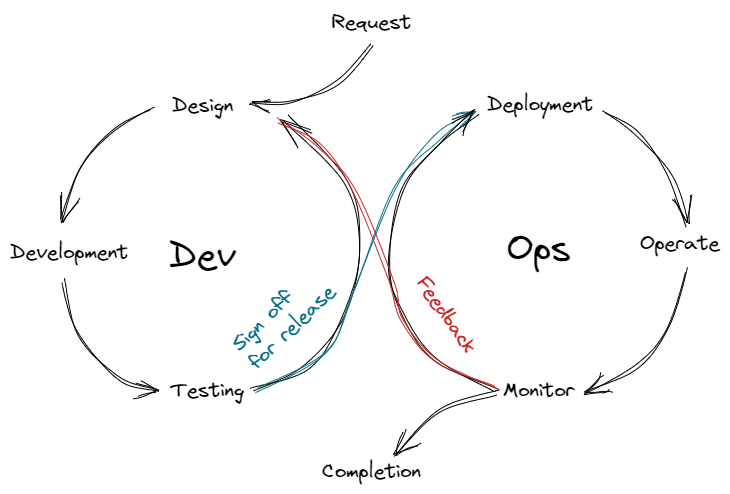
\includegraphics[width=350pt]{chapters/ap/figures/cd.png}
	\caption{CI and CD.} \label{ch:cicd:fig:cd}
\end{figure}

Under the framework of CI/CD in Fig. \ref{ch:cicd:fig:cd}, the developer not only develops the new feature, but also integrates the features with the help of version control and branch management tool Git, compiles the packages using build server, deploys the new packages in the testing environment by preparing machine-readable instruction files, and finally tests the new features using pre-configured test cases in the machine-readable testing scripts.

Since the operation team joins the developers team, they are now called the DevOps team. The CI/CD framework shown in Fig. \ref{ch:cicd:fig:cd} is known as the CI/CD pipeline which represents an end-to-end software development lifecycle (SDLC) within its ecosystem.

This CI/CD framework enables fast deployment of new packages. Large IT companies can make up to dozens of new releases everyday.
